\documentclass[dvipdfmx,autodetect-engine, unicode, 10pt, aspectratio=169]{beamer}

% \documentclass[dvipdfmx,autodetect-engine]{jsarticle}
% \usepackage{luatexja}% 日本語
% \usepackage[haranoaji,deluxe]{luatexja-preset}% フォント指定
\renewcommand{\kanjifamilydefault}{\gtdefault}% 既定をゴシック体に

\usetheme[progressbar=frametitle]{metropolis}
\usepackage{appendixnumberbeamer}
\usepackage{booktabs}
\usepackage[scale=2]{ccicons}
\usepackage{pgfplots}
\usepgfplotslibrary{dateplot}
\usepackage{xspace}
\newcommand{\themename}{\textbf{\textsc{metropolis}}\xspace}
\usepackage{adjustbox}
\usepackage{caption}
\captionsetup[figure]{font=tiny}
\usepackage{fancyvrb} % verbatim replacement that allows latex
\usepackage{listings} % Setting for Code block
\usepackage{bm} % for Bold font in Math \bm

\title{多変量解析}
\subtitle{証券アナリスト}
% \date{\today}
\date{}
\author{Takayuki Suzuki}
\institute{This is institude of the author}

\begin{document}

\maketitle


\begin{frame}{多変量解析目標}
    線形代数(ベクトルと行列)では、「理解する」と「計算できる」が有る。 
    \begin{itemize}
        \item 主成分分析の行列計算との対応
        \item 主成分分析の主成分ベクトルの意味が説明できる
        \item 主成分得点が計算できる
        \item 因子分析と主成分分析の違いが説明できる
        \item バリマックス回転?プロマックス回転?
        \item 判別分析、クラスター分析、マハラノビス距離などの用語を知っている
    \end{itemize}
    計算できる必要があるのは、2x2の固有方程式から固有ベクトルを計算すること \\
    および対角化、そして、関数を成分とするベクトルの微分表記、計算ができること。 \\
\end{frame}

\begin{frame}{出る問題}
    結局、例の、水準(パラレルシフト)、傾き、曲率の問題に落ちる。\\
    この問題について、主成分分析にフォーカスして解説する。
    例えば、水準はたいていの場合第一主成分だが、なぜ第一主成分なのか?など。
\end{frame}

\begin{frame}{主成分分析}
    \small
    多変数からなるデータを分析する手法。\\
    データを分析するとき、変数同士に相関が無い方が分析しやすい。  \\
    また、データの変動に影響が有る変数の順番が分かっていた方が分析しやすい。\\
    しかし、一般的にデータは変数同士は相関があるし、どの変数が最も影響があるか、明らかではない。\\
    主成分分析を行うと、1.互いに独立で、2.最も影響がある変数から順番に、新しい変数を作ることができる。

    \begin{minipage}{0.45\linewidth}\scriptsize
        右は、主成分分析のイメージ。
        x,yの二つの変数のデータから、新しい軸(茶軸)を作る。\\
        元のデータは、x,yで表現されると、相関がある。(斜めの傾向が見える)\\
        しかし、新しい軸で見ると、相関が無いデータになる。\\
        しかも、最も変動が大きい方向が第一主軸となっている。\\
        主成分軸は、それぞれ直交する。さらに、元となったデータは、元の軸には相関があったが、主成分軸で表現すると、相関のないデータになっている。これは主成分を用いる最も大きなメリットである。
    \end{minipage}
    \begin{minipage}{0.45\linewidth}
        \begin{figure}[h]
        \centering
            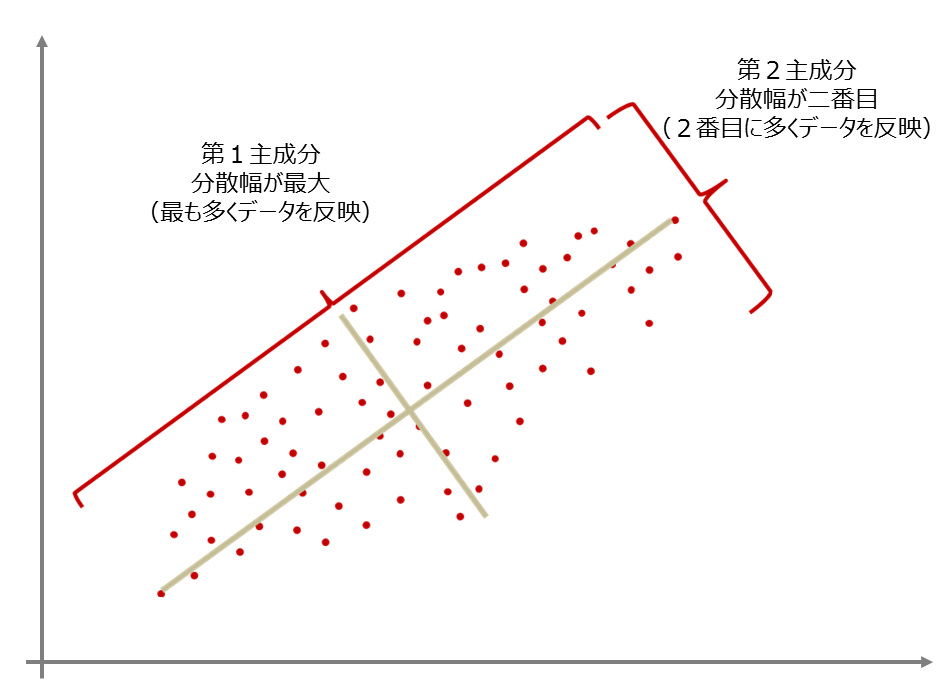
\includegraphics[width=0.9\textwidth]{PCA.png}
        \caption*{\tiny https://www.intage.co.jp/glossary/401/}
        \label{fig:mesh1}
        \end{figure}
    \end{minipage}
\end{frame}

\begin{frame}{主成分分析の計算方法}
    主成分分析は、データをよく表現する新しい変数を作る事。どうやって作る?\\
    ⇒ 元の変数の分散共分散行列の固有値と固有ベクトルを求めればよい (覚える)\\
    \vspace{10pt}
    例えば、ある2変数$x_1, x_2$からなるデータが有って、それぞれの変数の分散が$\sigma^2_{x_1}=4, \sigma^2_{x_2}=7$, 共分散が$\text{cov}(x_1, x_2)=2, \text{cov}(x_2, x_1)=2$であったとき(共分散は順番が変わっても同一であるから、分散共分散行列は常に対称行列である)、これを主成分分析する例を考える。
\end{frame}
\begin{frame}{主成分分析の計算方法}    
    主成分分析を計算するには固有値、有ベクトルを求めればよい。 \\
    $
        \text{分散共分散行列} = 
            \begin{bmatrix}
                \sigma^2_{x_1} && \text{cov}(x_1, x_2) \\
                \text{cov}(x_2, x_1) && \sigma^2_{x_2}
            \end{bmatrix} = 
            \begin{bmatrix}
                4 && 2 \\
                2 && 7
            \end{bmatrix}
    $ \\
    前章の手順に従い固有値と固有ベクトルを求めると、\\
    固有値は$\lambda = 8, 3$, 対応する固有ベクトルは\\
    $\bm{w}_1 = \begin{bmatrix}
        1/\sqrt{5} \\ 2/\sqrt{5}
    \end{bmatrix}$
    および
    $\bm{w}_2 = \begin{bmatrix}
        2/\sqrt{5} \\ -1/\sqrt{5}
    \end{bmatrix}$
    であることが分かる(計算せよ)\\
    絶対値が大きい固有値8に対応するベクトル$\bm{w}_1$が第一主軸で、\\
    固有値3に対応するベクトル$\bm{w}_2$が第二主軸である。
\end{frame}

\begin{frame}{主成分得点}
    この主軸はどのように使うか?\\
    あるサンプルA(サンプルというのは、データの中の一点のこと)を考える。
    $A\sim \bm{x}_A = (x_1, x_2) = (3, 2)$というデータが有ったとする。主成分分析では、
    このデータを新しい軸(主成分軸)でとりなおすことを行う。\\
    新しい軸での各成分のことを、第一主成分得点、第二主成分得点などという。
    \begin{align*}
        &A = \begin{bmatrix}
            3 \\
            2
        \end{bmatrix}
        &\Longrightarrow \hspace{30pt}
        &A = \begin{bmatrix}
            \text{第一主成分得点} \\
            \text{第二主成分得点}
        \end{bmatrix} \\
        &\text{\footnotesize もとの軸での表現} &\text{    }  &\text{\footnotesize 主成分分析で作られた新しい軸での表現}
    \end{align*}
    \\
    上記は2次元の場合であるが、3次元以上の場合もしばしば問題に出る。(水準、傾き、曲率) 
\end{frame}
\begin{frame}{主成分得点の計算方法と例}
    主成分得点は、元のベクトルを各主軸への射影成分を取ることで得られる。\\
    射影は、内積を取ることで得られる。
        \begin{align*}
        A\sim \bm{x}'_A = 
        \begin{bmatrix}
            \text{第一主成分得点} \\
            \text{第二主成分得点}
        \end{bmatrix} &=
        \begin{bmatrix}
            \text{Aの第一主軸への射影成分} \\
            \text{Aの第二主軸への射影成分}
        \end{bmatrix} \\
        & =
        \begin{bmatrix}
            \bm{w}_1\cdot \bm{x}_A \\
            \bm{w}_2 \cdot \bm{x}_A
        \end{bmatrix} \\
        & = \begin{bmatrix}
            \frac{7}{\sqrt{5}} \\ \frac{4}{\sqrt{5}}
        \end{bmatrix}
    \end{align*}
    これが、新しい軸でのデータAの表現である。(上記結果になることを確認せよ)

\end{frame}

\begin{frame}{元のデータの再現}
    主成分得点から元のデータを再現する方法は計算できるようにしておく。
    \begin{align*}
        A &= \frac{7}{\sqrt{5}}\bm{w}_1 + \frac{4}{\sqrt{5}}\bm{w}_2 \\
          &= \frac{7}{\sqrt{5}}\begin{bmatrix}
              1/\sqrt{5} \\
              2/\sqrt{5}
          \end{bmatrix} +
          \frac{4}{\sqrt{5}}  \begin{bmatrix}
              2/\sqrt{5} \\
              -1/\sqrt{5}
          \end{bmatrix}\\
          &= \begin{bmatrix}
              7/5 \\
              14/5
          \end{bmatrix} +
          \begin{bmatrix}
              8/5 \\
              -4/5
          \end{bmatrix}  \\
          &= \begin{bmatrix}
              15/5 \\
              10/5
          \end{bmatrix} \\
          &= \begin{bmatrix}
              3 \\
              2
          \end{bmatrix}
    \end{align*}
\end{frame}

\begin{frame}{寄与率}
    主成分には、それぞれ寄与率というものがある。\\
    それぞれの主軸の寄与率は、各主軸に対応する固有値を、すべての固有値の和で割ることで求められる。 \\
    先ほどの例では、第一主成分の固有値が8, 第二主成分の固有値が3であったので
    \begin{align*}
        \text{第一主軸の寄与率}=\frac{8}{8+3} = \frac{8}{11}\simeq 0.73 \\
        \text{第二主軸の寄与率}=\frac{3}{8+3} = \frac{3}{11} \simeq 0.27
    \end{align*}
    そもそも、寄与率は、そのデータの分散(データの動き)のなん%がその軸で説明できるかを表している。
    上記例の場合、データの動きの約73\%が第一主軸だけで説明できるということになる。\\
    第一主軸はデータの分散が最も大きい方向を示すベクトルであるから、寄与率も最も大きくなる。
\end{frame}

\begin{frame}{その他の解析手法}
    \begin{itemize}
        \item 因子分析は、分析の際に、\underline{\textbf{モデルを仮定する}}ことが、主成分分析との違い。
        \item 判別分析は、教師あり学習の一つで、対象サンプルの属するグループ(\underline{\textbf{クラス)}})を推定する方法
        \item 回帰分析は、判別分析と対になるもので、対象サンプルの持つ何らかの\underline{\textbf{数値}}を推定する方法
        \item クラスター分析は、\underline{\textbf{教師なし学習}}の一つで、データをいくつかのグループに分ける方法
    \end{itemize}
\end{frame}
\end{document}
